\chapter{Introduction}
\label{chap:ps_introduction}

The increasing availability of always-connected smartphone devices has led to their use for a multitude of applications. In this first part of the thesis, we focus on research and deployed mechanisms that use smartphones to enhance the security of other applications, such as unlocking cars, entering buildings and ticketing.

In the solutions that we present in the following chapters we always have similar design goals; security, usability and deployability. Security plays an important role both in two-factor authentication for the web and in payments at points of sale. On the web, large-scale leaks of database passwords~\cite{yahoohack,linkedinhack,evernotehack} render two-factor authentication a strong mechanism to prevent attackers from gaining unrestricted access to users' online profiles and data. When it comes to payments at points of sale, targeted attacks against stolen credit cards information account for over 1 billion Euros of frauds in the Euro zone alone~\cite{ECB2012}. Similarly, a two-factor authentication mechanism can be used to prevent these fraudulent transactions.

The typical use-case for two-factor authentication on the web is to perform an extra verification of a user trying to log in to a web server. In general, the idea is that the user supplies his username and password (what he knows) and then inputs a one-time-code that proves the possession of an external device (the second factor). While for most sites this happens only upon login, services that require stronger security guarantees might ask the user to supply the information generated on the external device multiple times (e.g., when issuing a bank transfer). In Figure~\ref{fig:2fa} we show a schematic view of a login transaction in both cases when two-factor authentication is absent and when it is present.

\begin{figure}[!ht]
    \centering
    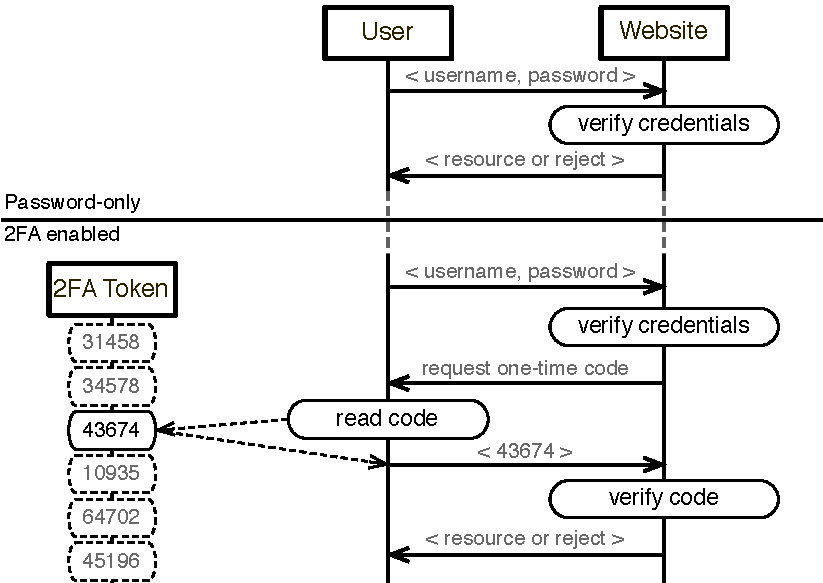
\includegraphics[width=.9\linewidth]{figures/phonesecures/intro_2fa}
    \caption[Web login without 2FA and with 2FA enabled]{Overview of a web login operation in the absence (top) and presence (bottom) of a generic two-factor authentication mechanism.}
    \label{fig:2fa}
\end{figure}

While security plays an important role, we also stress usability and deployability as further goals of our work. A plethora of two-factor authentication mechanisms have been proposed for web authentication but a recent study~\cite{petsas15eurosec} has found that only 6.4\% of users actually use two-factor authentication for their e-mail accounts. While the scenario is different where two-factor authentication is mandatory (e.g., for banking institutions), the situation still looks grim in scenarios where the second factor is optional (e.g., access to e-mails, social networks, coding websites, online games, and online shopping portals).

One of the problems with current two-factor authentication schemes for the web is that they require user interaction~\cite{google_authentication,yubico,authy,encap}, for example to type into the browser a one-time-code received through SMS or from an application (as shown in Figure~\ref{fig:2fa}). Users have to find their smartphones, unlock them, open the application or wait for the SMS message to arrive, and then copy the code in order to log in. Proposed solutions that do not require user interaction leverage system resources that are not currently available to web browsers, such as bluetooth~\cite{czeskis12ccs} or direct access to the wireless network card of the system~\cite{shirvanian14}.

In Chapter~\ref{chap:ps_soundproof} we introduce Sound-Proof, a scheme that provides two-factor authentication for web logins by checking the proximity of the user's smartphone to the computer where he is logging in. We perform such a check by comparing audio simultaneously recorded by the smartphone's and the computer's microphones. If the two audio samples match, the user is successfully logged into the system. Sound-Proof is completely transparent to the user, making the login process similar to password-only authentication in terms of user experience. We evaluate Sound-Proof in different scenarios, both indoors and outdoors and show its applicability as well as its security against an attacker that is not co-located with the victim (as for most two-factor authentication schemes). In a user-study that compared Sound-Proof with Google 2 Step Verification, users ranked Sound-Proof considerably higher in terms of its usability. Similarly, participants appreciated the reduced time that Sound-Proof imposed on the overall login procedure, compare to the code-based approach. Finally, as Sound-Proof requires access to only the microphone on both devices it is deployable on major browsers as well as on Android and iOS smartphones.

In contrast to web authentication, improving the security of payment systems at points of sale requires a solution that can withstand a more targeted attack carried our by an attacker who has a high incentive to perform a fraudulent transaction. However, deployability and usability are still of paramount importance. On the one hand, users are not willing to change their behavior when purchasing goods with credit cards (that is, sign or enter a PIN code) nor are they willing to spend more time than necessary to finalize the purchase. On the other hand, payment terminals have restricted hardware support and offer only restricted interactions with the customer. Upgrading payment terminals to support a new secure scheme would be a long and costly process, impacted by requirements for standardization, proofs of correct implementation, and deployment.

In Chapter~\ref{chap:ps_tee} we propose a two-factor authentication solution for payments at points of sale that does not require the user to interact with his smartphone nor require extra software or hardware on the terminals. Our solution is secure against a strong attacker model that can mount targeted attacks and can compromise the user's phone remotely or fully compromise any phone to which he has physical access. We rely on the system-wide security offered by ARM TrustZone to perform a location verification when the user performs a payment at a point of sale. We propose two novel enrollment schemes for the application running in the secure world of the user's smartphone that guarantee security without relying on the trust-on-first-use assumption. Finally, we implement the proposed schemes on available hardware and show their deployability. Through a field study we verify that our proposed solution thwarts targeted attacks and further show how it can be applied to other scenarios that have similar requirements, such as entrance to buildings and public transport ticketing.